\section{Planificación de Implementación del Sistema}
En este plan se describirá como se llevará a cabo el despliegue del sistema, incluyendo publicidad, instalaciones , software, hardware y configuraciones.

Si bien ofrecemos una API pública y una interfaz web que facilita el uso a cualquier usuario, contemplamos que muchas de las instituciones necesitarán gestionar el sistema en un servidor propio. Por este motivo se ha desarrollado dicho documento que permitirá llevar a cabo de manera adecuada la correcta migración del sistema.

\subsection{Objetivo}


Ofrecer un sistema funcional que brinde la posibilidad de cargar la información necesaria para la utilización eficiente del sistema.
\subsection{Alcance}
\begin{itemize}
	\item Lograr la aceptación del público
	\item Instalación y configuración del servidor.
	\item Instalación y configuración de la base de datos
	\item Desplegar el web services.
	\item Carga inicial de datos
\end{itemize}

\subsection{Publicidad y propaganda}

Antes de comenzar a definir que técnicas utilizaremos, es necesario diferenciar a estos dos métodos. Por un lado, la publicidad es una herramienta que se utiliza con objetivos comerciales; en nuestro caso conseguir una venta. La propaganda por otro lado difiere de la publicidad, su objetivo es modificar ideologías, costumbres y la visión de la realidad, objetivo fundamental de nuestro sistema.

Invertiremos en realizar publicidad en aquellos sitios web de salud que lo permitan, para conquistar a aquellos usuarios interesados por su cuidado personal.

Utilizaremos lugares relacionados a la salud para dar a conocer nuestro producto, estos lugares pueden ser hospitales, farmacias, centros de salud, etc. Aprovecharemos la intima relación que tiene nuestro sistema con los lugares antes citados para establecer  convenios que permitan el beneficio mutuo  a partir de la prestación del servicio de nuestro sistema. 
Por ejemplo actualmente existen farmacias que brindan, a sus clientes, la posibilidad  de acceder a una cuenta para ver  los productos que se ha comprado a lo largo de su historia como cliente, dándoles puntos por cada compra que luego podrán canjear, sería interesante ofrecerle a esas farmacias nuestro sistema para que ellos le brinden a sus clientes mas beneficios y así nuestro sistema se beneficiaría con la popularidad del mismo.

También será necesario realizar una buena campaña de marketing utilizando propaganda en Youtube para atrapar a aquellos usuarios que no se encuentran familiarizados con la tecnología, pero que si se interesarán por los beneficios que ofrece nuestro sistema.

\subsection{Configuración y diseño del sistema}
Para facilitarle el acceso al usuario se implementará el sistema en una plataforma web utilizando un servidor diferente del servidor que gestionará las conexiones a la  API y a la base de dato.

Esta arquitectura del sistema se puede observar en la \textbf{[Figura \ref{esq_funcionamiento}]} en ella se puede ver como los dispositivos móviles que acceden a través de la aplicación tienen acceso directo a la capa de servicio a diferencia de aquellos que acceden al sistema a través del navegador que tiene acceso a la capa de servicio a través del servidor Web.

Esta topología será mejor a la hora de escalar para soportar y brindar servicio a los usuarios que lo requieran, sin incurrir en tiempos prolongados de espera ni modificaciones en la arquitectura y el diseño del sistema.


 \begin{figure}
  \centering
  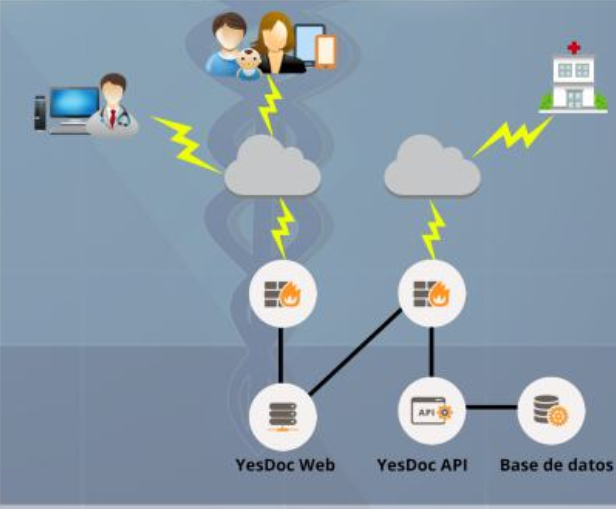
\includegraphics[width=.8\textwidth]{img/esq_funcionamiento}
  \caption{Arquitectura del sistema}
  \label{esq_funcionamiento}
\end{figure}


\subsubsection{Obtener DNS}
Registrar un dominio que represente a \textbf{``YesDoc''}, el cuál será utilizado entre otras cosas como url del Web Service.
Actualmente la web se encuentra hosteada en un subdominio de herokuapp. \textbf{``https://yesdoc.herokuapp.com''}

\subsubsection{Evaluar los costos y capacidades de servidores}
Se evaluaran los costos necesarios en cuanto a servidores para poder  cumplir con los requerimientos de una cantidad inicial de usuarios. Luego será incrementada la capacidad de los cosmos a medida que la cantidad de usuarios aumente. 

\subsubsection{Instalación y puesta en marcha de servidores}
Se instalará un servidor que permita desplegar angular y Flask con soporte para la base de     datos a utilizar. 

\textbf{Medida de seguridad}
\begin{itemize}
	\item \textbf{Redireccionar puerto 80: } Se implementará un filtro de redirección, para redirigir todas las peticiones http a puerto 80, con el fin de evitar intrusos en direcciones al servidor.
	\item \textbf{Implementación de HTTPS: } el sistema HTTPS utiliza un cifrado basado en SSL para utilizar un canal seguro.
	\item \textbf{Timeout: }Se trata del valor en segundos que esperará el servidor web en procesar peticiones de clientes, en el caso de que una petición tarde más tiempo del permitido, la respuesta que dará el servidor será un error de timeout. El timeout sirve para evitar peticiones con comportamiento extraño.
	\item \textbf{Prohibir que el servidor ingrese a directorios fuera de su raiz} permitirle que tenga acceso a directorios fuera de su raiz es dejar una gran brecha de seguridad, por lo cual es necesario evitarlo.
	\item \textbf{Implementar Mod\_Security:} Este es un Firewall de aplicaciones Web que puede manejar varias tareas incluyendo fitrado simple,filtrado de expresiones regulares, validación de la codificación de una URL, entre otras.
\end{itemize}

\subsubsection{Instalación y configuración de la base de datos}
	Se instalará la base de datos y configurará los usuarios, contraseñas y permisos de cada administrador.
	
	También se configurará a base de datos de manera que exista una réplica de la  misma en otro servidor, la cual entre en funcionamiento si la primera deja de funcionar.
	
	Por último se establecerán las políticas de backup necesarias.


	\subsubsection{Preparación de datos y archivos}
	Será necesario determinar cuál será la base de conocimiento que se cargará en el sistema, estas deberán cumplir con los estándares medicinales, algunos ejemplos son:
    \begin{itemize}
        \item Especialidades
        \item Tipos de  análisis
        \item Tipo de mediciones 
        \item Formatos de análisis
        \item Sobre el paciente: sexo, enfermedades, estados fisiológicos, etc.
        \item Información farmacológica: alergias, medicamentos.
        \item Productos comerciales: productos farmacéuticos que se comercializan en un área o región, nombre comercial, presentación, dosificación, precio, cobertura, tipo de dispensación, conservación, origen, laboratorio que lo produce. Las fuentes de donde se obtiene la información son la industria farmacéutica, financiadores de salud y farmacólogos clínicos. Estos datos son generalmente mantenidos por empresas abocadas a tal fin y en algunos casos por organismos oficiales encargadas de informar periódicamente a sus suscriptores sobre las altas, bajas o modificaciones de productos medicinales.
        \item Principios activos o monodrogas: nombre genérico, sinónimos, clasificación farmacológica y/o terapéutica, farmacodinamia y farmacocinética, preparación, formas de administración, rango de dosis recomendada, dosificación en pacientes pediátricos, dosificación en ancianos, dosificación en insuficiencia renal, dosificación en insuficiencia hepática severa, dosificación en cirrosis, embarazo y lactancia, sobredosis, precauciones, indicaciones, contraindicaciones, reacciones adversas, antagonismos y antidotismos, interacciones, efectos sobre exámenes de diagnóstico e información para los pacientes
        \item Terminología médica: Unified Medical Language System (UMLS); SNOMED CT  terminología clínica integral, multilingüe y codificada de mayor amplitud, precisión e importancia desarrollada en el mundo; variantes léxicas, opciones controladas, reglas terminológicas, CIAP-2 Clasificación Internacional de Atención Primaria.
        \item Prestadoras, aseguradoras, lugares físicos y prestaciones.
	\end{itemize} 
    
Además se deberá modelar el sistema para que permita futuras conexiones con otros similares ya existentes, como pueden ser de laboratorios o la historia clínica del hospital al que incurre el paciente que quiere utilizar el sistema. Es por este motivo que se ofrece una API que permita la conexión de sistemas ajenos al nuestro.


\subsubsection{Despliegue del servidor de front-end}
Para aquellas personas que deseen utilizar el sistema de manera particular, añadiendole funcionalidades y cambiando el diseño o las interfaces para que el tiempo de adaptación sea el mínimo, se presenta un documento detallado indicado la forma de desplegar el sistema localmente para que puedan evaluarlo y modificarlo como mas lo deseen.

Dichos pasos además de detallarse a continuación se encuentran en el archivo \textit{\textbf{README.md}} del proyecto que se encuntra hosteado en \textit{github}.
%siempre usando la API proporcionada desde un principio
\lstset{language=bash,breaklines=true, showspaces=false,showstringspaces=false, backgroundcolor=\color{background}}
\begin{enumerate}
\item \textbf{ Instalar NodeJS}

\begin{lstlisting}[language=bash]
curl --silent --location https://deb.nodesource.com/setup_0.12 | sudo bash -
sudo apt-get install --yes nodejs

\end{lstlisting}
\item \textbf{Instalar las dependencias}
\begin{lstlisting}[language=bash]
# Instalar el administrador de paquetes
sudo apt-get install npm
sudo npm install -g npm

# Dependencias de NodeJS
cd web/
sudo npm install
sudo npm install -g yo bower grunt-cli

# Dependencias de YesDoc
cd web/
bower install
\end{lstlisting}
\item \textbf{Iniciar el servidor}
\begin{lstlisting}[language=bash]
# Para iniciar el servidor
grunt serve
\end{lstlisting}


\end{enumerate}

\subsection{Método de conversión}
El método de conversión será directo ya que contemplamos dos grandes grupos:
\begin{itemize}
	\item Instituciones que posean un sistema funcionando y quieran utilizar la API de YesDoc para brindarles mayor servicios a sus clientes.
	\item Instituciones que deseen usar nuestra interfaz, porque no poseen un sistema.
\end{itemize}



\newpage
\subsection{Gantt}



\begin{figure}
	\centering
	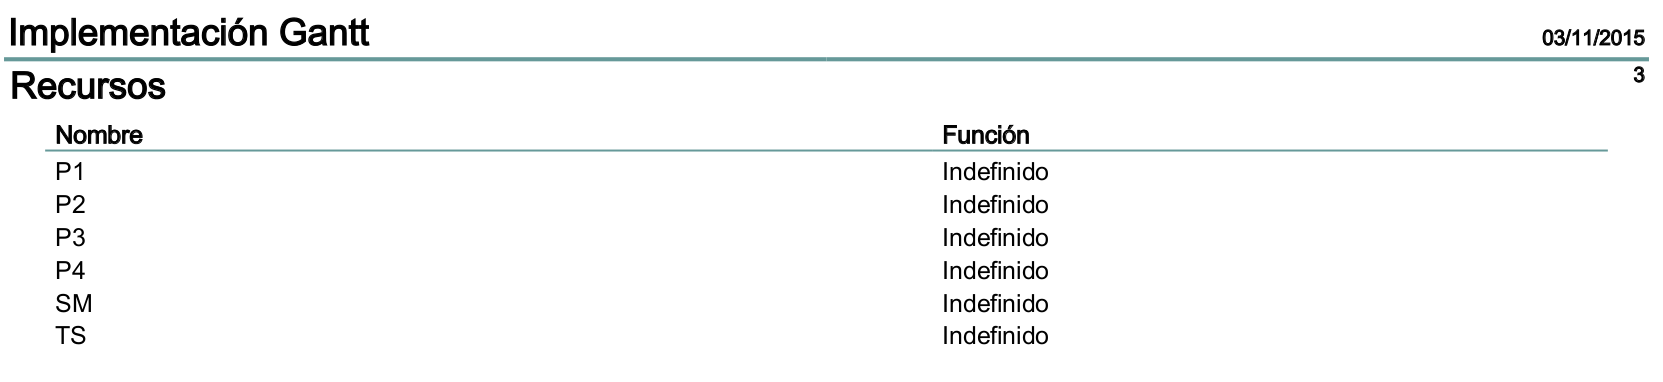
\includegraphics[width=.8\textwidth]{img/recursos_implementacion}
	\caption{Tareas necesarias para la implementación del sistema}
	\label{recursos_implementacion}
\end{figure}


\begin{figure}
	\centering
	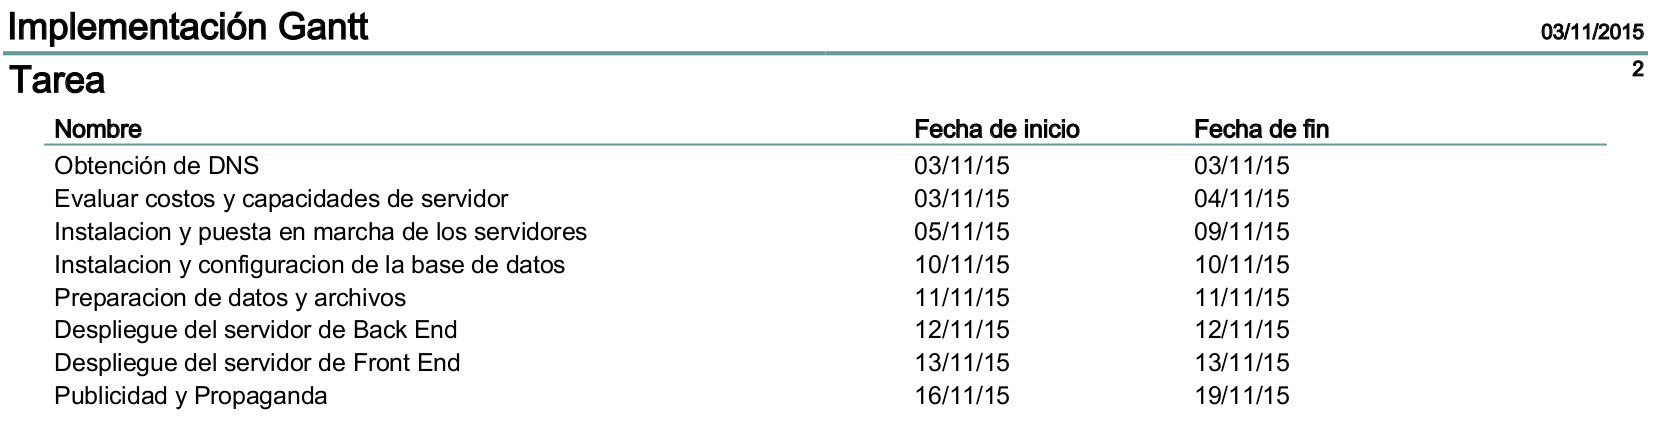
\includegraphics[width=.8\textwidth]{img/gantt_implementacion}
	\caption{Tareas necesarias para la implementación del sistema}
	\label{tareas_implementacion}
\end{figure}
\begin{figure}
	\centering
	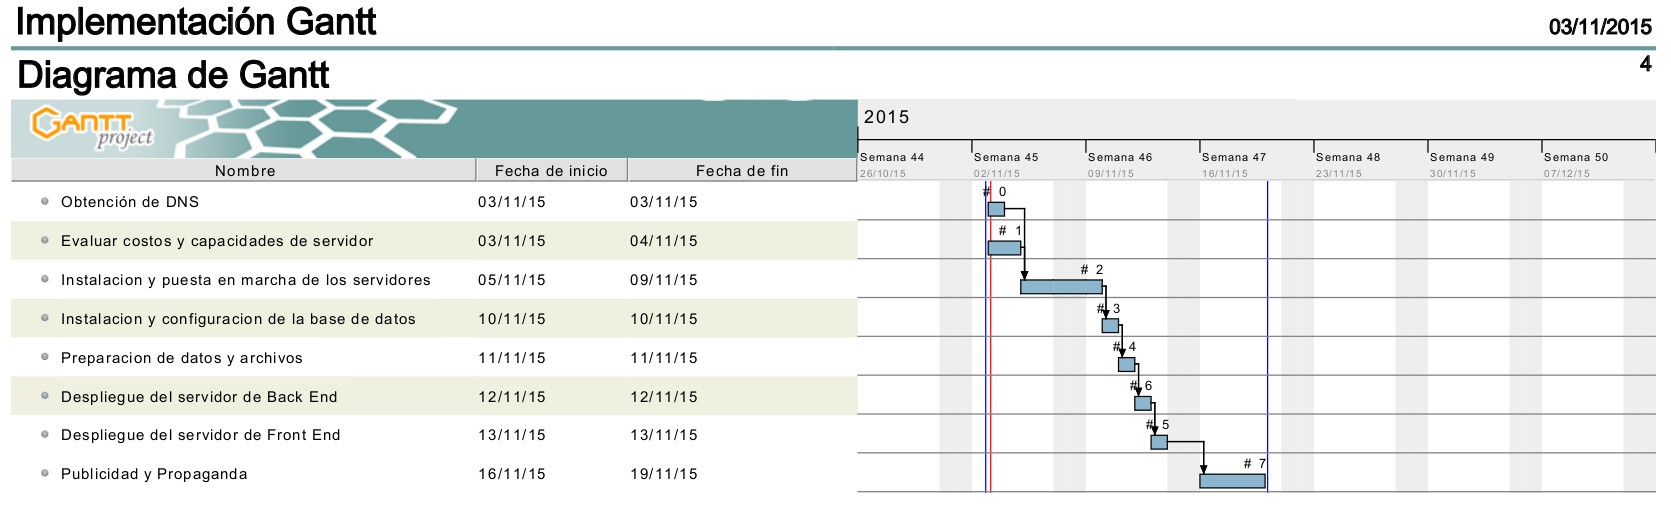
\includegraphics[width=.8\textwidth]{img/gantt_implementacion2}
	\caption{Gantt para la implementación del sistema}
	\label{gantt_implementacion2}
\end{figure}


\begin{comment}
http://velneo.es/cual-es-la-mejor-forma-de-vender-software-a-empresas-de-un-sector-especializado/
http://velneo.es/como-vender-programas-de-software/
http://velneo.es/segmentacion-de-mercado-en-software/
http://une-senn.tripod.com/new_page_3.htm
http://asistemgrp5.weebly.com/plan-de-conversioacuten.html
Método de conversión o implementación: directa, en paralelo, piloto, pruebas de versiones

Actividades: como hacer la publicidad, la promoción, como linquearlo, capacitación pilóto,  migracion de base de datos, configuración y diseño de red,
______________________________________________________________
Método de conversión del sistema, metodos, actividades y justificaciones. Siempre hay un sistema del que partimos, siempre hay una conversión de lo antiguo a lo actual. Directa, en paralelo, piloto.
Capacitación puede ser. Nuestro desafío es que la gente está muy encasillada en como se maneja con la salud, tenemos que ver como se lo vamos a hacer entrar. Antes la gente guardaba sus documentos de salud en un armario.
\end{comment}